\documentclass[a4,10pt]{article}

\usepackage{amsmath, amsthm, amssymb}
\usepackage[ansinew]{inputenc}
\usepackage{mathtools}
\usepackage{ulsy}
\usepackage{scrextend}
\usepackage[ampersand]{easylist}
\usepackage{enumerate}
\usepackage{pst-tree}
\usepackage{graphicx}
\newcommand{\HRule}{\rule{\linewidth}{0.5mm}}
\usepackage{titlesec}
\usepackage{pdfpages}

\addtolength{\oddsidemargin}{-.5in}
\addtolength{\evensidemargin}{-.5in}
\addtolength{\textwidth}{1in}
\addtolength{\topmargin}{-1in}
\addtolength{\textheight}{2in}
\setlength{\parindent}{0in}

\setcounter{secnumdepth}{4}

\titleformat{\paragraph}
{\normalfont\normalsize\bfseries}{\theparagraph}{1em}{}
\titlespacing*{\paragraph}
{0pt}{3.25ex plus 1ex minus .2ex}{1.5ex plus .2ex}

\begin{document}




\begin{titlepage}
\begin{center}
 

\vspace*{75mm}

{ \huge \bfseries Assignment \# 1 \\[0.4cm] }

\textsc{\LARGE CS 2731 }

\HRule \\[2.5mm]

{ \large Joseph Knittel }






\vfill

% Bottom of the page
{\large October 03, 2013}

\end{center}
\end{titlepage}















\section{Introduction}


Making observations about the current state of a system and using that knowledge to predict future states is a critical process in any scientific investigation. \\

In the realm of Natural Language Processing, N-gram models are frequently used to predict the next word in a sentence given a set of previous words. \\

However, the utility of these probabilistic models is not limited strictly to the scale of words. N-gram models can be built at the character level to describe the actual structure of the words themselves or they can even be built at the sentence level to get an idea of how paragraphs are composed in a document. \\

This paper describes the process of using character-based N-gram models to determine the most likely language in which a test document was written. Models are constructed using English, German, and Spanish training documents and the perplexity values observed from each model run on the test document are compared to give a reliable prediction of the test document's language.   


\section{Program}

A program was created in Python to build a suite of unsmoothed and smoothed N-gram models for English, German, and Spanish. \\

These models could then be used to compute perplexity values for a test document which, in turn, could be used to predict the test document's language. 

\subsection{Building the N-Gram Models}

The ``N" in N-gram signifies the length of the sub-components used to analyze the structure of the feature being investigated.  \\

In this paper, for instance, a 2-gram (commonly referred to as a ``bigram") would be a model that uses 2-character chunks of data to describe the structure of words in a document. \\

We start by constructing basic unigram (1-gram), bigram (2-gram), and trigram (3-gram) models for each language and then adjust them with smoothing techniques called Laplace smoothing and interpolation. 

\subsubsection{Basic (Unsmoothed) N-gram Models}

\paragraph{N-gram Counts}

The first step in constructing these basic N-gram models is to count all of the times each N-gram occurs in the training documents. \\

This was done by scanning through each training document one character at a time and storing (if it exists) the unigram, bigram, and trigram ending in the current character in a dictionary. \\

If the N-gram is already in a dictionary, then 1 is added to the value of the N-gram's key in the dictionary. \\

\textbf{Example}:  (current character =  `g') 
\begin{verbatim}   uni[`g'] = uni.get(`g') + 1 
\end{verbatim}

\newpage

Once the training documents have been scanned, the program adds in all N-grams that were not seen in the training documents into the dictionaries as 0 counts. \\

\textbf{Code}:

\begin{verbatim}
for i in uni:
        for j in uni:
            if not bi.has_key(i + j): bi.update({i+j:0})
\end{verbatim}

The above code is used to store 0 counts for every possible bigram that was not observed in the training documents. 

\paragraph{Computing MLE Probabilities}

Once N-gram counts are logged, they can be used to approximate the probability of a specific character occurring given a sequence of preceding characters. \\

The most basic estimate of this probability is the Maximum Likelihood Estimate (MLE). \\

The MLE states that the probability of a given future character occurring is just the count of that specific character preceded by some (n-1) characters divided by the count of all (n-1)-character strings that are equal to the first (n-1) characters in the numerator. \\

This can be more clearly understood in equation form: 

\begin{equation} P(u_n | u^{n-1}_{n-N+1}) = \frac{C(u^{n-1}_{n-N+1}u_n)}{C(u^{n-1}_{n-N+1})} \end{equation}

where $C$ stands for the N-gram count and $u$ stands for unit (in our case, character) \\

The previously recorded N-gram counts were used in this calculation to compute unsmoothed unigram, bigram, and trigram models of the training documents. 

\subsubsection{Smoothed N-gram Models}

Unsmoothed N-gram models give the most basic approximation of the probability that a specific character might occur given some preceding characters. However, significant issues arise when an N-gram occurs in the test document and not in a training document. Namely, division by zero occurs which yields an undefined probability for the given character. \\

To avoid this situation, smoothing techniques are used to re-distribute probability mass from more commonly occurring N-grams to the N-grams that were not observed in the training data. 

\paragraph{Laplace Smoothing}

The first smoothing method used was developed hundreds of years ago by the famous mathematician Pierre-Simon Laplace. \\

He suggested that we can update the probability from Equation 1 by just adding 1 to each of the N-gram counts and then dividing the result by (the previous denominator + V) where V is, in our case, the total unique characters.   \\

This can be seen in Equation 2 below:

\begin{equation} P_{Laplace}(u_i) = \frac{c_i+1}{N+V} \end{equation}

\newpage

Observe the code below where Laplace smoothing was implemented in the program by adding 1 to the unsmoothed English trigram count and dividing by (the bigram count of the first two characters + the total unique English characters). \\

\textbf{Code}:
\begin{verbatim}
for i in uniENG:
    for j in uniENG:
        for k in uniENG:
            laplaceENG.update({i+j+k: \
            1. * (triENG[i+j+k] + 1) / (biENG[i+j] + len(uniENG))})
\end{verbatim}

\paragraph{Interpolation}

Another technique used to avoid the undefined probabilities that might arise with unsmoothed N-gram models is called interpolation. \\

Interpolation uses the key insight that although some higher-order N-gram counts might be zero, there are lower-order N-grams with non-zero counts that we can use in a weighted sum to approximate the probability given in Equation 1. \\

For the trigram probability, this can be stated as: 

\begin{align}
\hat{P} (u_n|u_{n-2}u_{n-1}) &= \lambda_1 P(u_n|u_{n-2}u_{n-1}) \nonumber \\
 &+ \lambda_2  P(u_n|u_{n-1}) \nonumber \\
 &+\lambda_3 P(u_n)
\end{align}

where all $\lambda$s sum to 1: 

\begin{equation} \sum_{i=1}^{3} \lambda_i = 1 \nonumber \end{equation}

The code below demonstrates how the interpolation smoothing method was implemented in the program for a Spanish trigram model. More sophisticated techniques optimize the values of the $\lambda$s, but for this paper each $\lambda$ was simply given the value $\frac{1}{3}$. \\

\textbf{Code}: 

\begin{verbatim}
for i in uniSPA:
    for j in uniSPA:
        for k in uniSPA:
            interpolatedSPA.update({i+j+k:(lambda1 * unsmoothTriSPA[i+j+k] 
                                         + lambda2 * unsmoothBiSPA[j+k] 
                                         + lambda3 * unsmoothUniSPA[k])})
\end{verbatim}

\subsection{Perplexity}

Once the unsmoothed and smoothed N-gram models were built, they could be put to work on a test document to predict the probability that a given sequence of characters might occur in a document. \\

The N-gram models were evaluated by how well they could guess the next character given a sequence of preceding characters. 

\newpage

In Natural Language Processing, this value is given by the perplexity of the character on a given N-gram model: 

\begin{equation} PP(u) = \sqrt[N]{\prod_{i=1}^{N}\frac{1}{P(u_i | u_1 \dots u_{i-1})}} \end{equation} 

The perplexity of a given character using an N-gram model is actually a weighted branching factor, therefore the model with the lowest perplexity value is the one which can best guess which character will come next given a sequence of preceding characters. \\

Perplexity was implemented in the program by scanning through the characters of a test document one by one and updating the perplexity value according to Equation 4. \\

The code below describes how the perplexity was calculated for the Laplace-smoothed German trigram model.\\

\textbf{Code}:

\begin{verbatim}
    LGpp = LGpp * pow(laplaceGER[curTri],norm)
\end{verbatim}

where this line of code was executed on each successive trigram in the test document \\
and norm $= \frac{1}{N}$ where N is the number of characters in the test document. 

\subsection{Output}

Given the perplexity values of each trigram model, the program should be able to evaluate which language the test document is written in. \\

To do this, I decided that smoothed models would be more accurate and therefore the program's language selection should thus be determined strictly based on the smoothed models' perplexitiy values. \\

I figured that both the Laplace and interpolation methods should be weighted evenly, therefore the chosen language is based on the minimum of the sum of Laplace and interpolation perplexities for each language.  \\

This was implemented with the following code. \\

\textbf{Code}: 

\begin{verbatim}
smoothENG = LEpp + IEpp
smoothGER = LGpp + IGpp
smoothSPA = LSpp + ISpp

if   smoothENG < smoothGER and smoothENG < smoothSPA: 
        print "The document is probably written in English!"
elif smoothGER < smoothENG and smoothGER < smoothSPA: 
        print "The document is probably written in German!"
elif smoothSPA < smoothENG and smoothSPA < smoothGER: 
        print "The document is probably written in Spanish!"
else:   print "The models were inconclusive in determining the language of the document."
\end{verbatim} 

\newpage

\subsection{Important Design Decision}

It is worth noting that the program was written exclusively for usage in CS 2731 class. \\

Therefore, the code was written to run with little input from the user. \\

\begin{addmargin}[2em]{0em}

\textbf{``python ngrams.py test"} will do the following: \\ 

1. Build N-gram models, and  

2. Evaluate the models to determine the language of the test document \\

\end{addmargin} 

In the real world, it would make far more sense to have the program only build the N-grams models once and output the models to files where they then could be used to evaluate any future test document, saving the user considerable time. \\

Since this program will likely only ever be used to determine the language of the provided test document, I found it to be reasonable to not generate additional files and both build the N-gram models and evaluate the test document all in one run.

\section{Test}

With a suite of unsmoothed and smoothed trigram models built for English, German, and Spanish languages, I decided to test their efficacy in predicting the source language of a document. \\

The figure below shows the program's output after examining the test document:

\begin{figure}[hb]
  \centering
  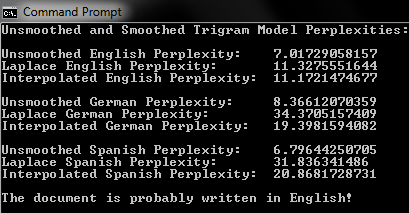
\includegraphics{output}
\end{figure}

\section{Critical Analysis}

So, a program was created to build N-gram models for different languages and then the N-gram models were used to evaluate the perplexity of a test document. \\

Using these perplexities, it was determined that the test document was written in English, but how can we be sure? \\

Some questions come to mind:  \\

\begin{addmargin}[2em]{0em}

\begin{enumerate}[(1)]

\item Why are these perplexity values a good indicator of the test document's language?
\item The program outputs nine perplexity values. Which ones are most valid?
\item Why does the program not consider unigram models and bigram models when determining the test document's language? 

\end{enumerate}

\end{addmargin}

\subsection{Perplexity as Indicator of Test Document's Language}

As stated in Section 2.2, perplexity, as it relates to N-gram models, is a measure of the average branching factor from a given sequence of preceding units to a following unit. \\

In the case of this investigation, perplexity = 1 would represent that the given model always knows exactly which character should follow a set of preceding characters. \\

Conversely, perplexity = 30 means that on average the model would predict any one of 30 possible characters to be the next one given a set of preceding characters. Clearly, this a model with perplexity = 30 is not as good at predicting future characters as a model with perplexity = 1! \\

So perplexity in this investigation is a good way to see how well a model can predict the next character in a document given a set of preceding characters, but what does this have to do with the language the document was written in? \\

Well, since the models were based on different languages (English, German, and Spanish), then their perplexity (i.e. their ability to predict a following character) is essentially the same thing as their ability to predict the structure of the words in the test document. \\

Therefore, if perplexity for a given model is low, then the model's language is probably the same as the test document's language!

\subsection{Unsmoothed vs. Smoothed N-gram Models}

A quick examination of the figure in Section 3 shows that perhaps the best model (lowest perplexity value) was the unsmoothed Spanish trigram model. \\

Why, then, does the program output that the test document is ``probably written in English"? \\

The reasoning behind this conclusion is based on the fact that when training data is limited or when the model is particularly sparse, unsmoothed N-gram models do not do a very good job at predicting future units, in general.  \\

Seeing as the Spanish training data has about 169,950 characters and the test document has about 13,801 characters, it can be assumed that the training data is somewhat limited in this case.\\

Additionally, Figure 1(a) shows probability values for all trigrams starting with the bigram `th' using the unsmoothed English trigram model.  Although the model in question is the unsmoothed Spanish trigram model, it can easily be checked that a similarly high percentage of all possible Spanish trigrams have a zero probability and hence are poor predictors of the actual language of the test document. \\

These findings as well the fact that smoothed N-gram models are better models than unsmoothed models in general led me to decided to use the sum of the perplexity values of the Laplace and interpolated models as the predictor of the test document's language.   

\subsection{Lower-Order N-gram Models vs. Higher-Order N-gram Models}

Finally, one might wonder why only the selected trigram models were used to determine the language in which the test document was written. \\

\newpage

The figure below indicates that unigram and bigram models produced significantly higher perplexity values than the trigram model: 

\begin{figure}[hb]
  \centering
  \includegraphics{unsmoothed}
\end{figure}

This is in accordance with what the textbook says about lower-order N-gram models being less precise and it makes sense too. \\

The larger the N-gram, the more previous information there is to be used to predict future characters and hence the better the model of the language's structure.  \\

Therefore, only trigram models were considered in the evaluation of the test document's language.

\section{Afterward}

The following section, Supplementary Figures, contains figures showing the requested printouts for the assignment. \\

Figure 1 displays the probabilities for all three trigram models of all trigrams starting with `th' \\

Figure 2 demonstrates that the three trigram models for English do indeed sum to 1 and hence are true probability distributions



\newpage

\section{Supplementary Figures}

\begin{figure}[hb]
  \centering
  \includegraphics[scale = 0.55]{th+}
  \caption {A printout of all trigrams probabilities for the (a) Unsmoothed English trigram model, (b) Laplace-smoothed English trigram model, and (c) Interpolation-smoothed English trigram model. It is clear to see that smoothing removes probability mass from common trigrams and adds it to less common trigrams. Also, note that in all models, the vast majority of probability mass is attributed to the trigram `the' because obviously the word ``the" is a trigram which is seen very frequently in the English language.}
\end{figure}

\newpage

\begin{figure}[hb]
  \centering
  \includegraphics[scale = 0.60]{sums}
  \caption {To ensure that each model constructs a valid probability distribution, the sum of all possible trigrams given some bigram should equal 1. In this case, sums were calculated for the (a) English Unsmoothed trigram model, (b) English Laplace-smoothed trigram model, and (c) English Interpolation-smoothed trigram model all given a preceding bigram `th'. All models did, indeed, sum to 1 indicating that the models do produce valid probability distributions over trigrams. }
\end{figure}


\end{document}













































